\documentclass{article}
\setlength{\parskip}{5pt} % esp. entre parrafos
\setlength{\parindent}{0pt} % esp. al inicio de un parrafo
\usepackage{amsmath} % mates
\usepackage[sort&compress,numbers]{natbib} % referencias
\usepackage{url} % que las URLs se vean lindos
\usepackage[top=25mm,left=20mm,right=20mm,bottom=25mm]{geometry} % margenes
\usepackage{hyperref} % ligas de URLs
\usepackage{graphicx} % poner figuras
\usepackage[spanish]{babel} % otros idiomas
\usepackage[utf8]{inputenc}
\author{Angel Gonzalez Melendres \\Alfredo Cárdenas Mena\\Aarón Lozano A\\Daniel Garcia R\\Angel Mario Acalá R} % author
\title{Investigacion } % titulo
\date{\today}

\begin{document} % inicia contenido

\maketitle % cabecera

\begin{abstract} % resumen
En esta actividad se realizó una gráfica la cual describe el comportamiento acerca de cómo se comporta la aproximación al número pi, utilizando el programa python, también se vio lo que es el método Monte Carlo y cómo se puede utilizar.
\end{abstract}

\section{Introducci\'{o}n}\label{intro} % seccion y etiqueta
El motivo de esta tarea es obtener el número pi mediante en método Montecarlo pero con la ayuda de phyton así obteniendo también las gráficas del comportamiento que se va obteniendo de este al tomar varios valores hasta llegar a un valor aproximado de pi, el método Montecarlo o también llamado la simulación de Monte Carlo,o una simulación de probabilidad múltiple, es una técnica matemática que se utiliza para estimar los posibles resultados de un evento incierto. El método de Monte Carlo fue inventado por John von Neumann y Stanislaw Ulam durante la Segunda Guerra Mundial para mejorar la toma de decisiones en condiciones de incertidumbre. Su nombre proviene de un conocido casino en Mónaco, ya que el elemento del azar es el núcleo del enfoque de modelado, similar a un juego de ruleta.


\section{Desarrollo}

La simulación de Monte Carlo predice un conjunto de resultados con base en un rango estimado de valores frente a un conjunto de valores de entrada fijos. En otras palabras, una simulación de Monte Carlo crea un modelo de posibles resultados aprovechando una distribución de probabilidades, como una distribución uniforme o normal, para cualquier variable que tenga una incertidumbre inherente. Posteriormente, vuelve a calcular los resultados una y otra vez, cada vez utilizando un conjunto diferente de números aleatorios entre los valores mínimo y máximo. En un experimento de Monte Carlo típico, este ejercicio puede repetirse miles de veces para producir un gran número de posibles resultados.
El simulador monte Carlo tiene muchas ventajas respecto a otro tipo de análisis deterministas o de “estimación de un solo punto”. Entre ellos podemos destacar:

-Ofrece resultados gráficos. Gracias a los datos que genera una simulación Monte Carlo, es fácil crear gráficos de diferentes resultados y las posibilidades de que sucedan. Esto es importante para comunicar los resultados a otras personas interesadas.
-Análisis de sensibilidad. En este método resulta más fácil ver qué variables introducidas tienen mayor influencia sobre los resultados finales.
-El análisis de escenario. Usando la simulación Monte Carlo, los analistas pueden ver exactamente los valores que tienen cada variable cuando se producen ciertos resultados. Esto resulta muy valioso para profundizar en los análisis.
-Correlación de variables de entrada. También permite modelar relaciones interdependientes entre diferentes variables de entrada. Esto es importante para averiguar con precisión la razón real por la que, cuando algunos factores suben, otros suben o bajan paralelamente.
\begin{figure} [htp]% figura
    \centering
    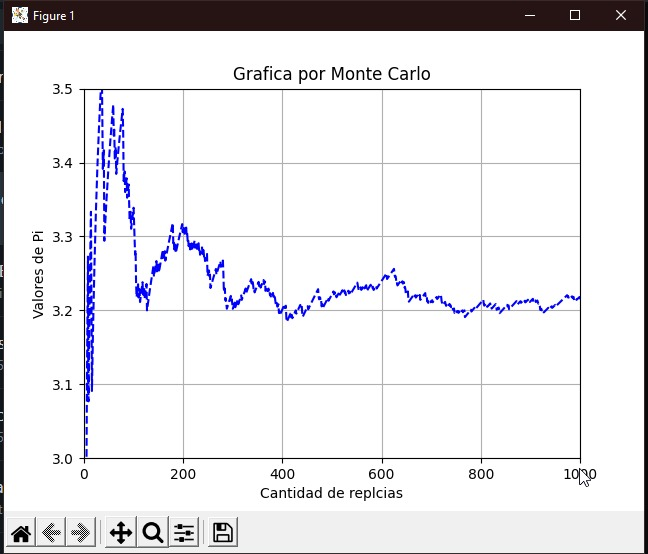
\includegraphics[width=140mm]{grafica.jpeg} % archivo
    \caption{Código con aproximamiento a n=1000}
    \label{grafica}
\end{figure}

\section{Conclusiones}
El método Montecarlo es una gran herramienta no nomás para el área científica sino también para el área de finanzas y otras cosas más, es una herramienta muy útil que nos ayuda aproximarnos a un valor requerido mediante muchas simulaciones obteniendo un valor más aproximado si hacemos más simulación, más sin embargo cómo en nuestro caso, solamente se aproxima al valor de pi pero no nos dará un valor exacto 

\section{Referencias}
\cite{Met}
\cite{Simul}
\bibliography{rfg.bib}
\bibliographystyle{apacite}

\end{document}